\chapter{Illumination optics}\label{chap:Illumination optics}
This chapter provides some concepts of illumination optics used in this thesis. We start explaining the difference between radiometry and photometry.
In particular, we focus on the photometric variables, defining them both in three and two dimensions. The reflection and refraction laws and the phenomenon of total internal reflection are explained next. The last paragraph of the chapter gives a brief introduction to Fresnel reflection. 
\section{Radiometric and photometric variables}\label{sec:photometry}
Radiometry concerns with the measurement of electromagnetic radiation across the entire electromagnetic spectrum. Photometry is the sub-field of radiometry that takes into account only part of the electromagnetic spectrum corresponding to the visible light \cite{zalewski1995radiometry}. Radiometry deals with radiometric quantities. An important radiometric quantity  is the radiant flux $\Phi_{\textrm{r}}$ (unit watt \textrm{W}) which is the total energy emitted from a source or received by a target per unit time:
\begin{equation}
\Phi_{\textrm{r}} = \frac{\textrm{d}Q}{\textrm{d}\mytime}\,,
\end{equation}
where $Q$ is the energy and $\mytime$ the time.\\
\indent In illumination optics the measurement of light is given in terms of the impression that it gives on the human eye. Therefore, illumination optics deals with photometric variables rather than with radiometric variables. The most important photometric variables are defined in the following using the notation adopted by Chaves in \cite{chaves2015introduction}. The luminous flux $\Phi$ (unit lumen, \textrm{lm}) is defined as the \textit{perceived} power of light by the human eye.
 The radiant and the luminous flux are related by the luminous efficacy function $y$ (unit \textrm{lm}/\textrm{W}) which defines how many lumen correspond to one Watt of power at a given wavelength.
 The luminous efficacy function reaches its maximum  at a wavelength of $555$ $\textrm{nm}$ where it is equal to $683$ $\textrm{lm}/\textrm{W}$.
  We may normalize the luminous efficacy function with its maximum value of $683$.
  The normalized function $\bar{y}(\lambda)$ is the luminosity function shown in Figure $\ref{fig:luminosityfunction}$ where $\lambda$ is the wavelength. It is a \textit{dimensionless} quantity with a range between $0$ and $1$ \cite{schubert2005light}.
\begin{figure}[t]
%\label{fig:luminousfunction}  
  \begin{center}
  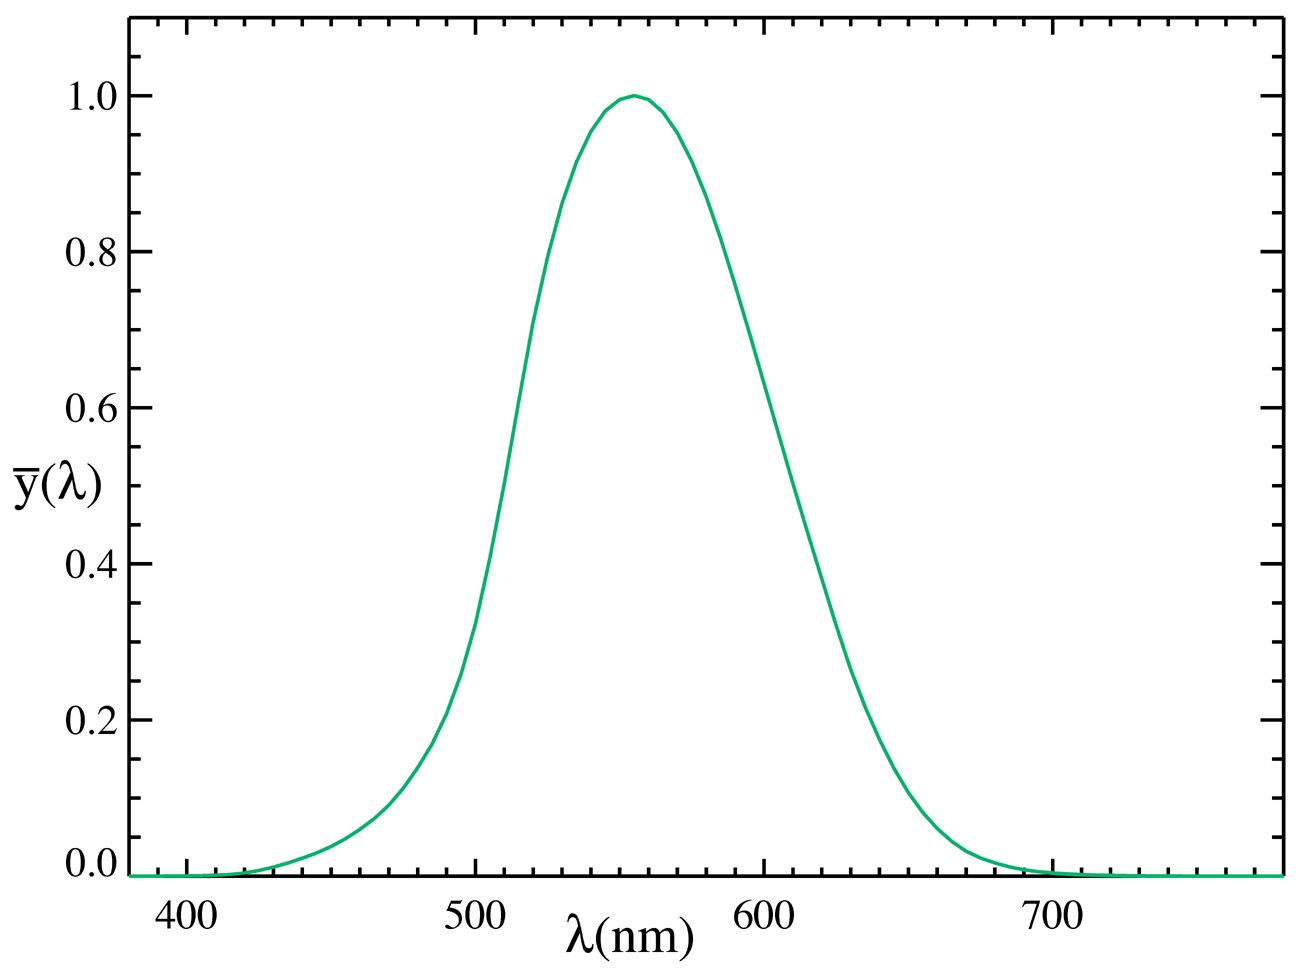
\includegraphics[width=7cm]{CIELuminosity}
  \end{center}
  \caption{\textbf{Luminosity function $\bar{y}(\lambda)$}. Relation between the eye's sensitivity and the wavelength of light. The luminosity function is dimensionless  \cite{wiki}.}
  \label{fig:luminosityfunction}
  \end{figure}
\\ \indent The luminous flux corresponding to one Watt of radiation power at any wavelength is given by the product of $683$ $\textrm{lm/W}$ and the luminosity function at the same wavelength,
i.e., $683 \, \bar{y}(\lambda)$. Hence, the total luminous flux $\Phi$ is defined as:
\begin{equation}\label{eq:luminous_flux}
\Phi = 683 \int_0^\infty \Psi_\textrm{r}(\lambda) \bar{y}(\lambda)\textrm{d}\lambda,
\end{equation}
where $\Psi_\textrm{r}(\lambda)$ is the spectral radiant flux, i.e., the power (in Watt) per unit wavelength (unit \textrm{W}/\textrm{m}). The corresponding photometric variable is the spectral luminous flux $\Psi(\lambda)$ (unit \textrm{lm}/\textrm{m}), i.e., the flux as perceived by the human eye as a function of the wavelength. 
Using the following relation between $\Psi_\textrm{r}$ and $\Psi$:
\begin{equation}
683 \bar{y}(\lambda) = \frac{\Psi(\lambda)}{\Psi_\textrm{r}(\lambda)}, 
\end{equation}
(\ref{eq:luminous_flux}) can be written as:
\begin{equation}
\Phi = \int_0^\infty \Psi(\lambda)\textrm{d}\lambda.
\end{equation}
%% Explain while integrals between 0 and infinity
%The luminous emittance $M = M(\vect{x}, \myangle)$ is the total flux emitted in all direction from a unit area. It is measured in lumens pr square meters (\textrm{lm}/$\textrm{m}^2$).
\\ \indent Geometric optics describes a beam of light as a collection of parallel light rays, where a light ray can be interpreted as a line or curve along which the electromagnetic energy travels. A ray is always direct perpendicular to the light's wavefront.  
The infinitesimal luminous flux $\textrm{d}\Phi$ incident on an infinitesimal surface $\textrm{d}A$ is called illuminance $E$ (unit $\textrm{lm}/\textrm{m}^2$)
and is defined as:
\begin{equation}
 E=E(\vect{x}) = \frac{\textrm{d}\Phi}{\textrm{d}A}\;.
 \end{equation}
The corresponding radiometric variable is called \textit{irradiance}, we indicate it with $P$. The density of light emitted by a point source in a given direction depends on the solid angle.\\ \indent
The solid angle in a given direction is expressed by a cone of rays emitted in that particular direction by a point source located at the center of the unit sphere \cite{koshel2012illumination}. Let us now consider a finite source $\textrm{d}A$ and let $\textrm{d}S$ be the area on the unit sphere subtended by the cone,
the infinitesimal solid angle $\textrm{d}\Omega$ is given by:
\begin{equation}\label{solid_angle}
\textrm{d}\Omega = \textrm{d}S= \sin(\theta)\textrm{d}\theta \textrm{d}\varphi,
\end{equation}
 where $\myangle$ and $\varphi$ are the polar and the azimuthal angle, respectively, which the normal $\boldsymbol{\nu}$ to the infinitesimal area $\textrm{d}A$ makes with the direction of the central line of $\textrm{d}\Omega$ (see Figure \ref{fig:rad}).
The solid angle on the entire unit sphere is $\Omega = 4\pi$ and its unit is steradian ($\textrm{sr}$) \cite{arecchi2007field}.
The luminous intensity $I$ (unit candela, $\textrm{cd}=\textrm{lm}/\textrm{sr}$) is defined as the luminous flux $\textrm{d}\Phi$ per solid angle
$\textrm{d}\Omega$ and is given by:
\begin{equation}\label{intensity}
I = I(\myangle, \varphi) = \frac{\textrm{d}\Phi}{\textrm{d}\Omega}\;.
\end{equation}
 \begin{figure}[t]
%\label{fig:cup}
  \begin{center}
  \includegraphics[width=6 cm]{SolidAngle}
  \end{center}
  \caption{\textbf{Solid angle}. $\textrm{d}\Omega$ is in a given direction $\myangle$ and $\varphi$.}
  \label{fig:rad}
  \end{figure}
\\ \indent 
The luminance $L = L(\vect{x}, \myangle, \varphi)$ (unit $\textrm{cd} / \textrm{m}^2$) depends both on the position and the direction, it is the luminous flux per unit solid angle $\textrm{d}\Omega$ and  per unit projected area $\cos\myangle \textrm{d}A$.  $L$  is given by:
\begin{equation}\label{luminance1}
  L=L(\vect{x}, \myangle, \varphi) = \frac{\textrm{d}\Phi}{\cos\myangle\textrm{d}A\textrm{d}\Omega}\,.
\end{equation}
\noindent Note that from ($\ref{intensity}$) and ($\ref{luminance1}$) we can derive a relation between the intensity and the luminance. 
The intensity $I$ emitted by the infinitesimal area $\textrm{d}A$ is given by:
\begin{equation}\label{eq:int_lum}
I = \frac{\textrm{d}\Phi}{\textrm{d}\Omega}= L(\vect{x},\myangle, \varphi)\cos\myangle\textrm{d}A \,.
\end{equation}
When the luminance is uniform over a finite area $A$, the luminous intensity emitted in the direction $\myangle$ and $\varphi$ is:
\begin{equation}
I(\myangle, \varphi) = L(\myangle, \varphi) A \cos\myangle\,.
\end{equation}
Further, when $L(\vect{x},\myangle, \varphi)$ does not depend on the position and the direction (i.e. $L(\vect{x},\myangle, \varphi)=L$), we obtain Lambert's cosine law:
\begin{equation}
I(\myangle) = I_0\cos\myangle ,
\end{equation}
where $I_0 = I(\myangle = 0) = LA$. Light sources emitting light with a constant luminance are called \textit{Lambertian} sources.\\
\indent Finally, we give a definition of the \'{e}tendue $U$ (unit $\textrm{m}^2\textrm{sr}$).
Etendue is a french word that means extent or spread. In geometric optics, it is a quantity to describe how light is spread out in terms of area and solid angle \cite{lerner2006etendue, zhu2011etendue}.
The quantity $ \textrm{d}U $ of a source $\textrm{d}A$ is defined as:
\begin{equation}\label{etendue}
\textrm{d}U = n^2  \frac{1}{L}\textrm{d}\Phi = n^2 \cos\myangle\textrm{d}A\textrm{d}\Omega,
\end{equation}
where $n$ is the index of refraction of the medium in which $\textrm{d}A$ is immersed. In phase space optics the \'{e}tendue is considered to be a volume in phase space (or an area for two-dimensional systems). This concept will be clarified in Chapter \ref{chap:PS} in which we treat the phase space in more detail.
An important property is conservation of \'{e}tendue within an optical system in the absence of absorption. 
In the following we show, using the approach of Chaves in \cite{chaves2015introduction}, 
how conservation of \'{e}tendue in a lossless system can be derived. 
%For the optical systems we will consider in this work, the source and the target are located in the same medium (air) with $n=1$, so the luminance $L$ equals the basic luminance $L^* = L/n^2$ at the source and the target of the system. 
Consider a light ray emitted from an infinitesimal area $\textrm{d}A_1$ to the area $\textrm{d}A_2$. Suppose that the centers of $\textrm{d}A_1$ and $\textrm{d}A_2$ 
are located at a distance \variabile{d} from each other and that both the surfaces are located in the same medium, see Figure \ref{fig:etendue_conservation}.
\begin{figure}[t]
 \label{fig:etendue_conservation}
     \begin{center}
     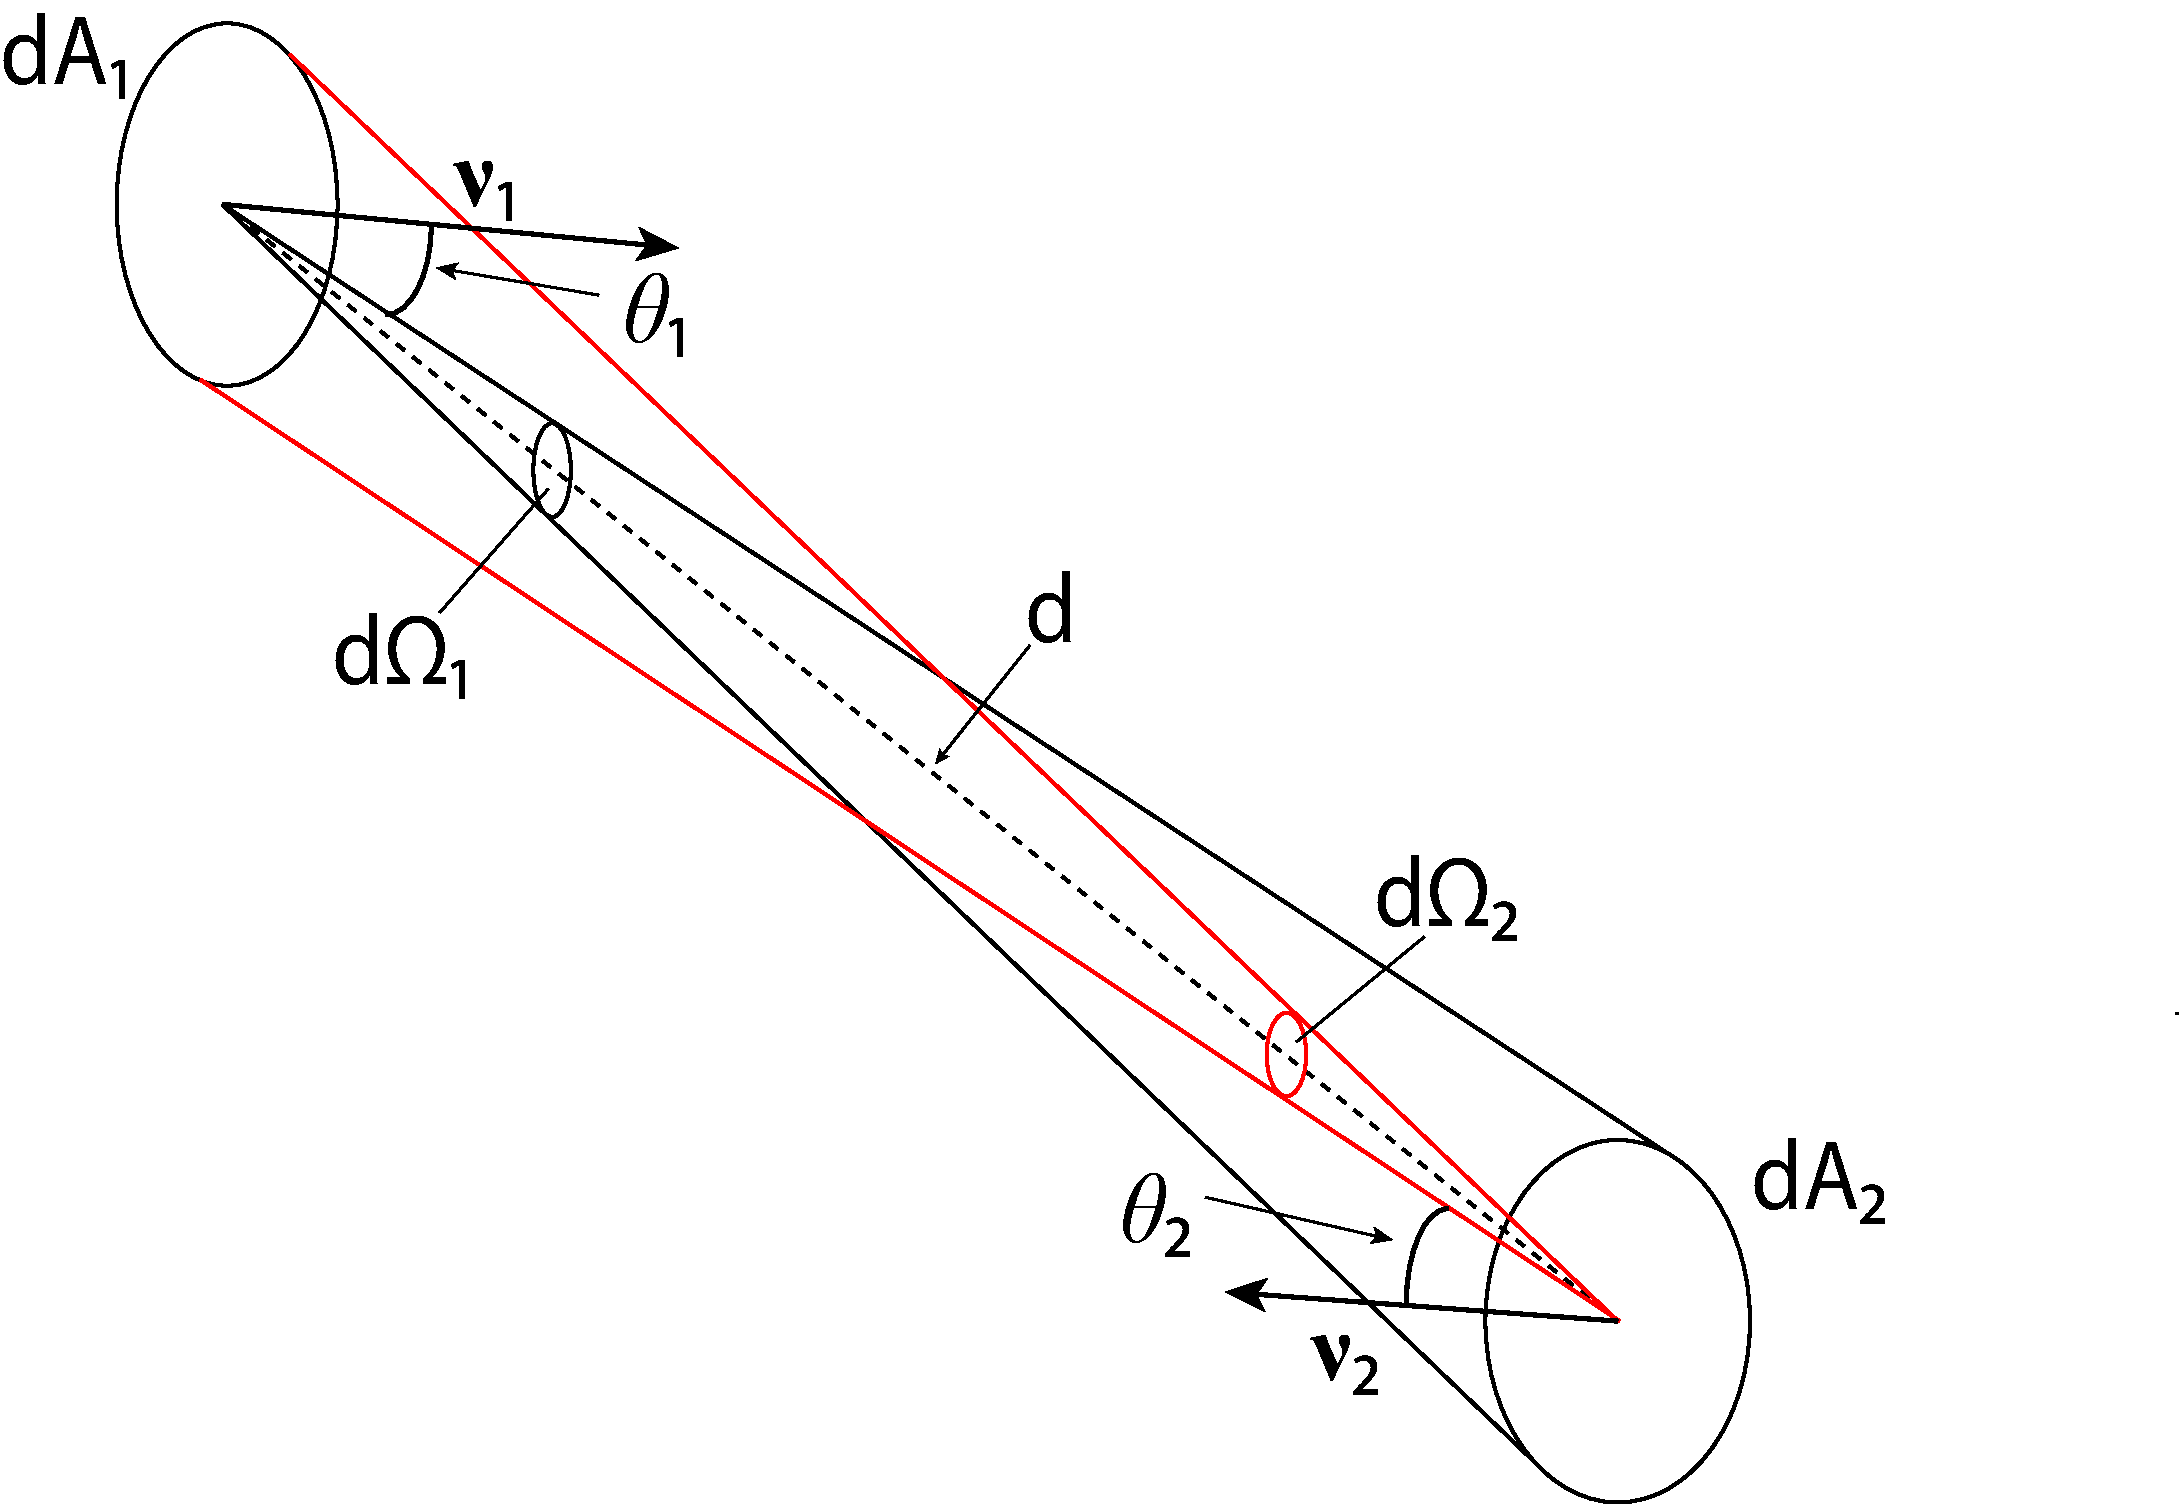
\includegraphics[width=10cm]{areas.pdf}
     \end{center}
     \caption{\textbf{Transfer of flux from the source $\textrm{d}A_1$ to the target $\textrm{d}A_2$.} $\textrm{d}A_1$ and $\textrm{d}A_2$ are two surfaces with normals $\nu_1$ and $\nu_2$, respectively. Their centers are located at a distance \variabile{d}.
$\myangle_1$ and $\myangle_2$ are the angles made by the central ray with the normals $\nu_1$ and $\nu_2$, respectively.}
\label{fig:etendue_conservation}
 \end{figure}
We derive \'{e}tendue conservation for the case in which $\textrm{d}A_1$ and $\textrm{d}A_2$ are located in the same medium (see \cite{chaves2015introduction, koshel2012illumination} for the general case).
We indicate with $\boldsymbol{\nu}_1$ and $\boldsymbol{\nu}_2$ the normals on the surfaces $\textrm{d}A_1$ and $\textrm{d}A_2$, and with $\myangle_1$ and $\myangle_2$ the angles that the ray connecting the centers of $\textrm{d}A_1$ and $\textrm{d}A_2$ forms with $\boldsymbol{\nu}_1$ and $\boldsymbol{\nu}_2$. The infinitesimal solid angle $\textrm{d}\Omega_1$ subtended by $\textrm{d}A_2$ at the center of $\textrm{d}A_1$ and the flux $\textrm{d}\Phi_1$ passing through $\textrm{d}A_2$ emitted from $\textrm{d}A_1$ are defined as:
\begin{subequations}
\begin{align}
\label{eq:omega1}
\textrm{d}\Omega_1 &= \frac{\textrm{d}A_2\cos(\myangle_2)}{\variabile{d}^2}\,,\\
\textrm{d}\Phi_1 &= L_1 \cos\myangle_1 \textrm{d}A_1 \textrm{d}\Omega_1. \label{eq:phi1}
\end{align}
\end{subequations}
Similarly, the infinitesimal solid angle $\textrm{d}\Omega_2$ subtended by $\textrm{d}A_1$ at the center of $\textrm{d}A_2$ and the flux $\textrm{d}\Phi_2$ passing through $\textrm{d}A_1$ emitted from $\textrm{d}A_2$ are equal to:
\begin{subequations}\begin{align}\label{eq:omega2}
\textrm{d}\Omega_2 &= \frac{\textrm{d}A_1\cos\myangle_1}{\variabile{d}^2}\,,\\
\textrm{d}\Phi_2 &= L_2 \cos\myangle_2 \textrm{d}A_2 \textrm{d}\Omega_2.\label{eq:phi2}
\end{align}
\end{subequations}
Then from (\ref{etendue}) we obtain the following relations: 
\begin{subequations}
\begin{align}
\textrm{d}U_1 &= n^2\cos\myangle_1 \textrm{d}A_1\textrm{d}\Omega_1= \frac{n^2\cos\myangle_1 \textrm{d}A_1\textrm{d}A_2\cos\myangle_2}{\variabile{d}^2},\\
\textrm{d}U_2 &= n^2 \cos\myangle_2\textrm{d}A_2\textrm{d}\Omega_2= \frac{ n^2 \cos\myangle_2\textrm{d}A_2\textrm{d}A_1\cos\myangle_1}{\variabile{d}^2}, \label{eq:dU2}
%\end{split}
\end{align}
\end{subequations}
for $\textrm{d}A_1$ and $\textrm{d}A_2$, respectively.
%From equation ($\ref{etendue1}$) and ($\ref{etendue2}$) 
From the previous equations we can conclude that $\textrm{d}U_1=\textrm{d}U_2$ and therefore the \'{e}tendue is conserved along a beam of light. 
Since the system is a lossless system, energy is conserved from the source to the target ($\textrm{d}\Phi_1= \textrm{d}\Phi_2$), therefore the \'{e}tendue conservation implies:
\begin{equation}\label{basicluminance}
L_1 = n^2 \frac{\textrm{d}\Phi_1}{\textrm{d}U_1} = n^2 \frac{\textrm{d}\Phi_2}{\textrm{d}U_2} = L_2\,,
\end{equation}
where the first equality comes from (\ref{luminance1}) combined with (\ref{etendue}).
\\ \indent In this thesis we consider two-dimensional optical systems. 
 Hence, the definitions of the photometric parameters have to be adapted to two-dimensions. An infinitesimal line segment of length $\textrm{d}\variabile{a}$ emitting a ray that makes an angle $\myangle$ with the normal $\boldsymbol{\nu}$ are considered, see Figure \ref{fig:2Dsolidangle}. 
\begin{figure}[t]
 \label{fig:2Dsolidangle}
     \begin{center}
     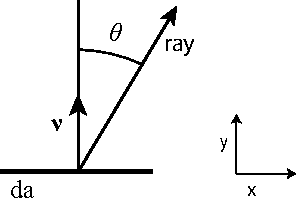
\includegraphics[width=7cm]{solidangle2D.pdf}
     \end{center}
     \caption{\textbf{Ray emitted by an infinitesimal line segment.} $\textrm{d}a$ makes an angle $\myangle$ with respect to the line normal $\boldsymbol{\nu}$.}
\label{fig:2Dsolidangle}
 \end{figure}
The two-dimensional illuminance (unit $\textrm{lm}/\textrm{m}$) denotes the luminous flux received by an infinitesimal line segment of length $\textrm{d}\variabile{a}$ 
and it is given by:
 \begin{equation}
 E=\frac{\textrm{d}\Phi}{\textrm{d}\variabile{a}}\;.
 \end{equation}
%The luminous emittance $M = M(\variabile{x}, \myangle)$ is the total flux emitted in all direction from a line segment.
The luminous intensity \big(unit $\big[\textrm{lm}/\textrm{rad}\big]$\big) is the luminous flux per angle $\textrm{d}\myangle$:
 \begin{equation}
 I=\frac{\textrm{d}\Phi}{\textrm{d}\myangle}\;.
 \end{equation}
 The two-dimensional luminance (unit $\textrm{lm}/(\textrm{rad}\,\textrm{m})$) is given by:
 \begin{equation}
 L= \frac{\textrm {d}\Phi}{\cos\myangle\,\textrm{d}\variabile{a} \,\textrm{d}\myangle}.
 \end{equation}
 Thus the following relation holds:
 \begin{equation}
 I = L(x, \myangle)\cos\myangle\,\textrm{d}\variabile{a},
 \end{equation}
where $x$ is a certain position at the light source $\textrm{d}\variabile{a}$. 
 Finally, the \'{e}tendue $\textrm{d}U $ (unit $\textrm{m}\;\textrm{rad}$) in two-dimensions is given by:
\begin{equation}\label{etendue2d}
\textrm{d}U = \n\cos\myangle\textrm{d}\variabile{a}\,\textrm{d}\myangle.
\end{equation}
An overview of the photometric variables used in this thesis is given in Table \ref{tab:photometric_variables}
\begin{table}[t] 
\centering
\caption{\bf Photometric variables}
\begin{tabular}{lllll}
 \hline   \\
Name  & Symbol & Unit ($3D$) & Unit ($2D$) \\
  \hline 
Luminous flux & $\Phi$   & $\textrm{lm}$   &  $\textrm{lm}$ \\
%Spectral luminous flux & $\Phi_\lambda$   & $$   &  $1.75\cdot10^{-4}$ \\
Illuminance/emittance  & $E$    & $\textrm{lm}/{\textrm{m}^2} $ & $\textrm{lm}/{\textrm{m}}$  \\
Intensity  & $I$    & $\textrm{lm}/{\textrm{sr}} = \textrm{cd}$  & $\textrm{lm}/\textrm{rad}$ \\
Luminance  & $L$  & $ \textrm{cd}/{\textrm{m}^2}$   & $\textrm{lm}/(\textrm{rad} \,\textrm{m})$ \\
Etendue & $U$  & $\textrm{m}^2\, \textrm{sr}$   & $\textrm{m}\, \textrm{rad}$ \\
 \hline
 \end{tabular}
\label{tab:photometric_variables}
 \end{table}
\\ \indent In order to determine the light distribution on a surface and to compute the photometric variables on that surface, we need to understand how the light emitted from a source propagates. In the field of geometric optics the light propagation is described by light rays.
The propagation of a light ray traveling through different media is determined by the reflection and refraction law.
In the following we introduce these two laws and we explain the total internal reflection phenomenon.
\section{Reflection and refraction law}\label{sec:reflection}
A light ray is described by a position vector \vect{x} on a surface and a direction vector \vect{t} and can be parameterized by the arc length \variabile{s}.
Light rays travel in a homogeneous medium along straight lines, once they hit a reflective surface their direction changes.
 Denoting with $\vect{t}_\textrm{i}$ the direction of the incident ray and with $\boldsymbol{\nu}$ the unit normal to the surface at the location of incidence, the direction $\vect{t}_\textrm{r}$ of the reflected ray is given by:
 \begin{equation}\label{Reflection}
  \vect{t}_\textrm{r} = \vect{t}_\textrm{i}-2 (\vect{t}_\textrm{i}\boldsymbol{\cdot}\boldsymbol{\nu})\boldsymbol{\nu},
\end{equation}
where the vectors $\vect{t}_\textrm{i}$ and $\boldsymbol{\nu}$ are unit vectors and $\vect{t}_\textrm{i}\boldsymbol{\cdot}\boldsymbol{\nu}$ indicates the scalar product of
$\vect{t}_\textrm{i}$ and $\boldsymbol{\nu}$. 
From the previous equation it follows that the vector  $\vect{t}_\textrm{r}$ is a unit vector too, indeed considering the scalar product $\vect{t}_\textrm{r}\boldsymbol{\cdot}\vect{t}_\textrm{r}$ we conclude:
\begin{equation}\label{unit_vector}
\vect{t}_\textrm{r}\boldsymbol{\cdot}\vect{t}_\textrm{r} = \vect{t}_\textrm{i}\boldsymbol{\cdot}\vect{t}_\textrm{i} 
- 4(\vect{t}_\textrm{i}\boldsymbol{\cdot}\boldsymbol{\nu})(\vect{t}_\textrm{i}\boldsymbol{\cdot}\boldsymbol{\nu})+
4(\vect{t}_\textrm{i}\boldsymbol{\cdot}\boldsymbol{\nu})^2(\boldsymbol{\nu}\boldsymbol{\cdot}\boldsymbol{\nu})=1 .
\end{equation} 
Note, from (\ref{Reflection}) that the vectors $\vect{t}_\textrm{i}$, $\vect{t}_\textrm{r}$ and $\boldsymbol{\nu}$ are coplanar.
Indicating with $\myangle_\textrm{i}$ the incident angle and with $\myangle_\textrm{r}$ the reflective angle such that $\myangle_\textrm{i}$, $\myangle_\textrm{r} \in[0, \pi/2)$,
the reflection law states that $\myangle_\textrm{i}=\myangle_\textrm{r}$, see Figure \ref{fig:Snell}.
\begin{figure}[t]
 \label{fig:Snell}
     \begin{center}
     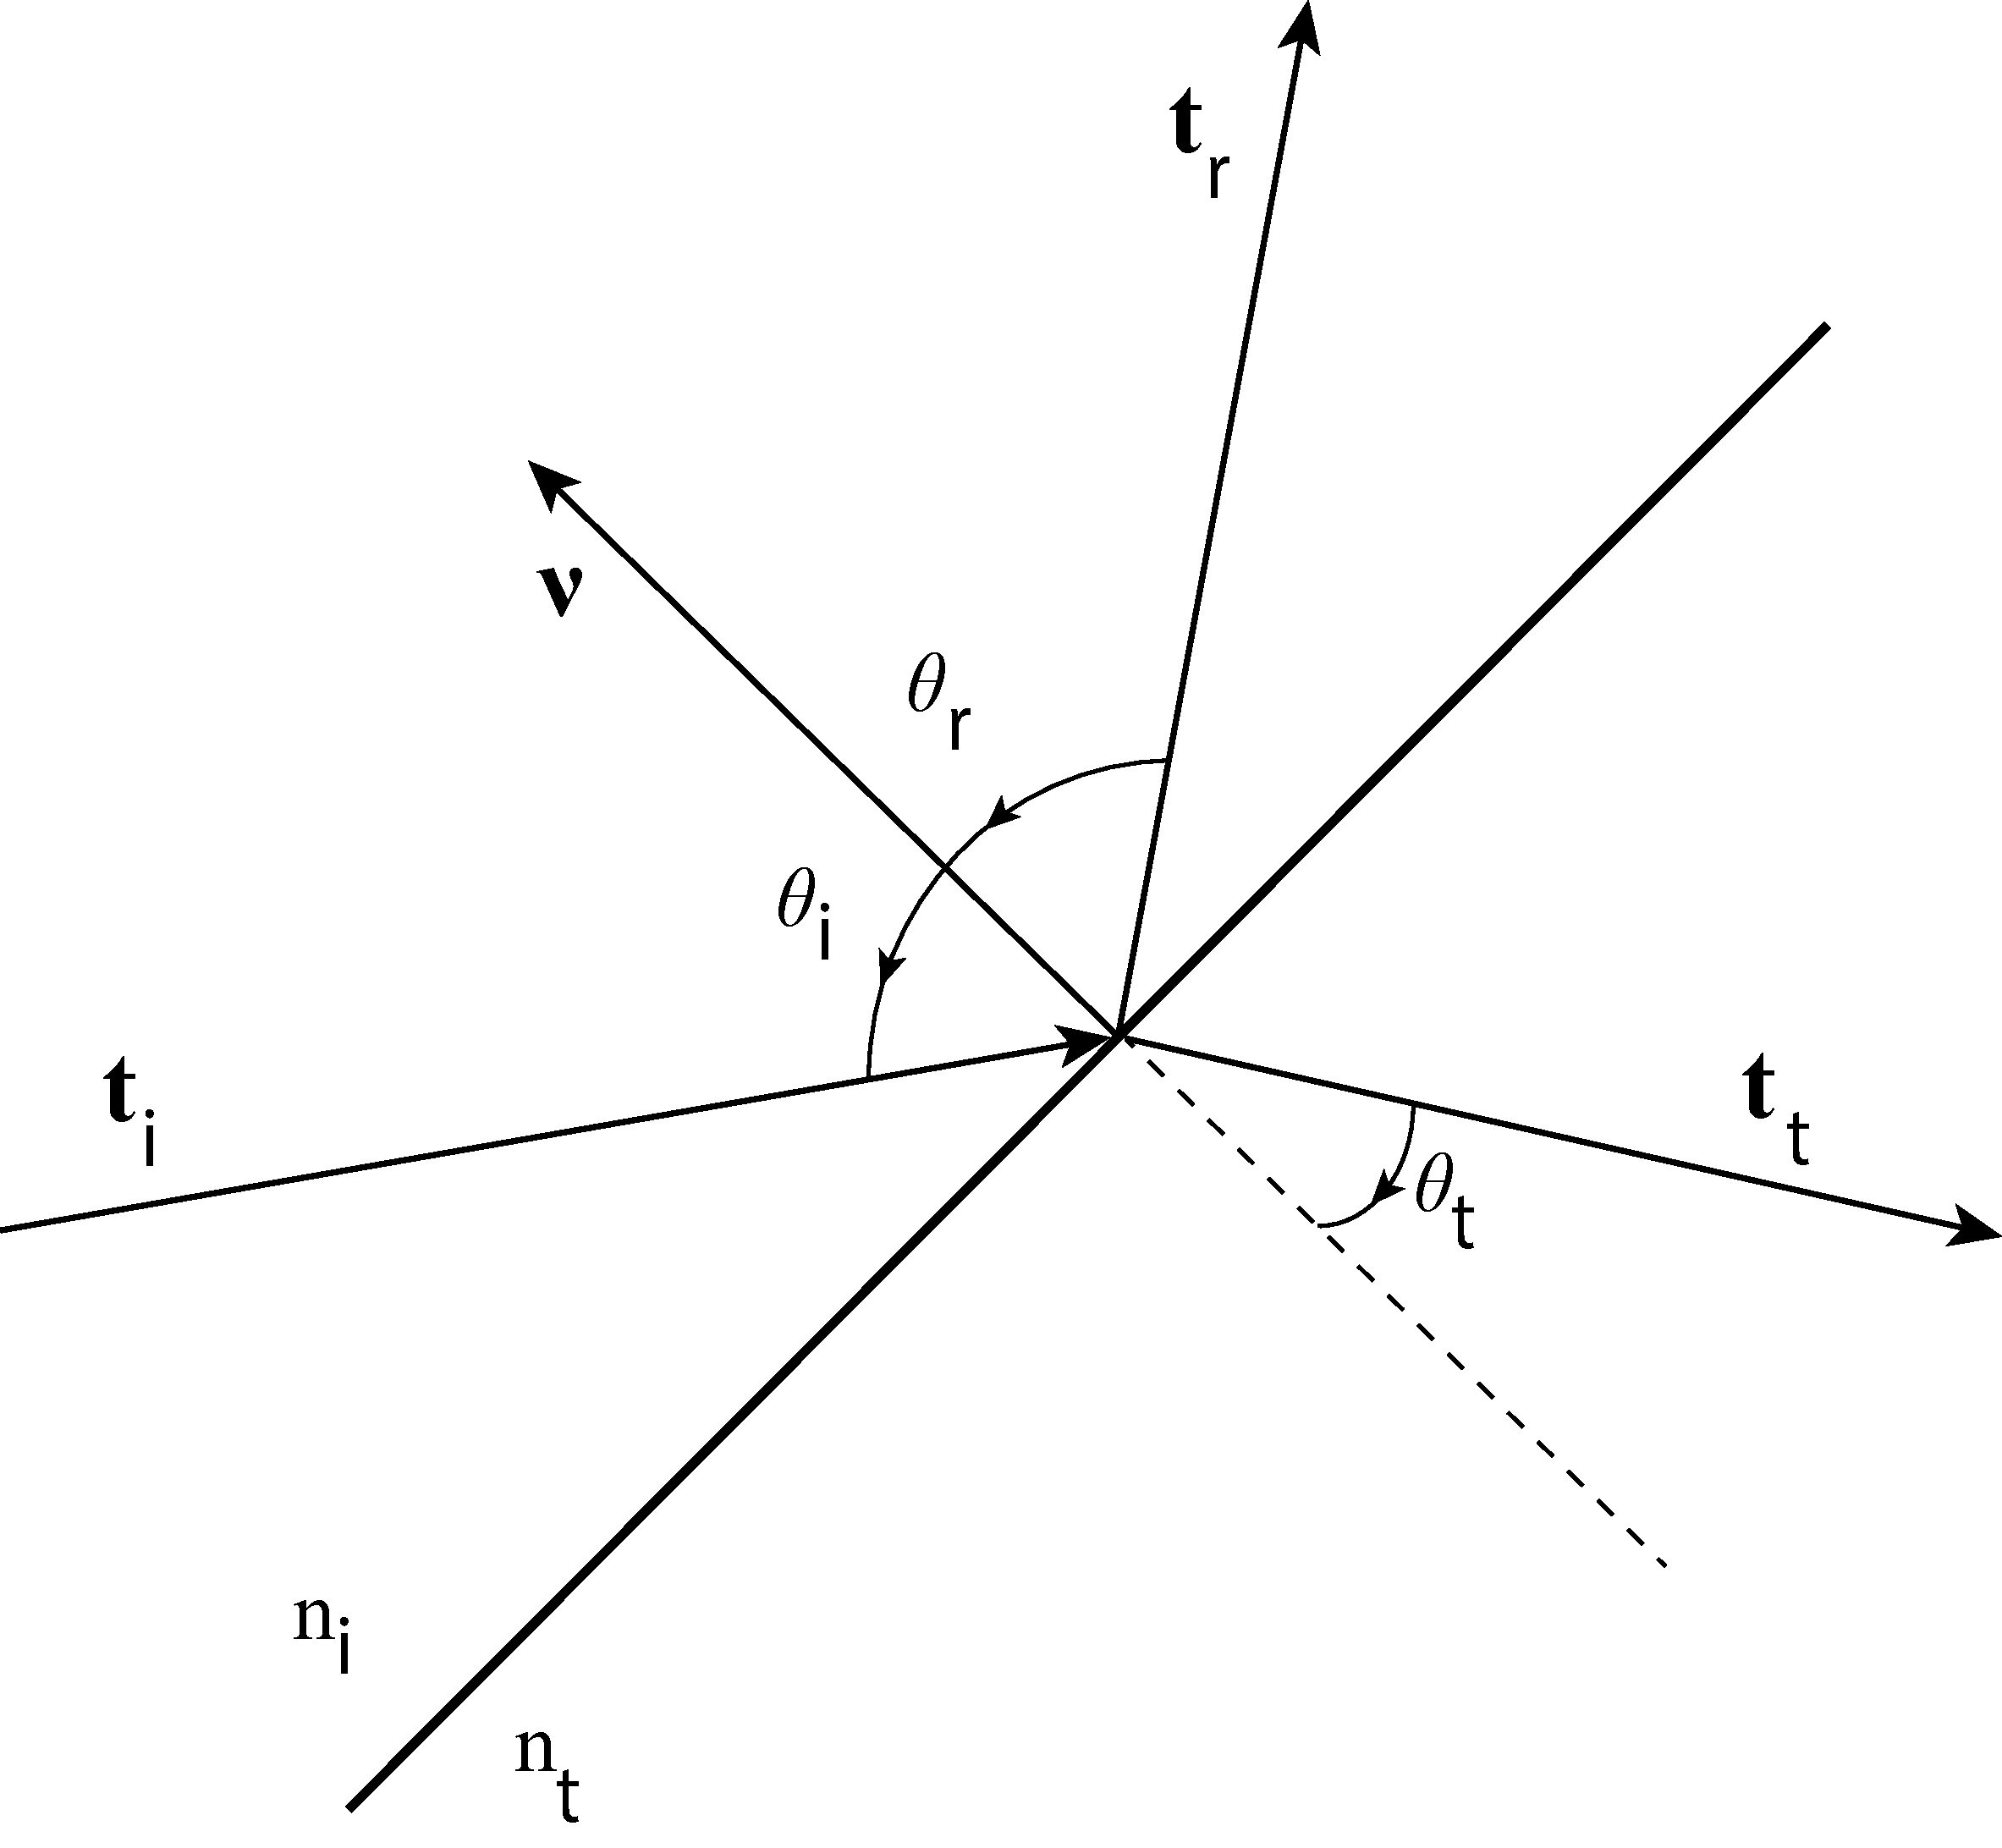
\includegraphics[width=8cm]{reflection}
     \end{center}
     \caption{\textbf{Propagation of a ray.} The ray travels through two materials with index of refraction $\n_\textrm{i}$ and $\n_\textrm{t}$.}% \bolsymbol{$\nu$} is the normal to the surface $A$ that the incident ray hits.
%$\vect{t}_i$, $\vect{t}_r$ and $\vect{t}_t$ are the direction vectors of the incident, reflected and refracted (or transmitted) ray, respectively. }}
%\myangle$_{i}$, \myangle$_{r}$ and \myangle$_{t}$ are the angles between \bolsymbol{$\nu$} and the incident, reflected and transmitted ray, respectively.}}
\label{fig:Snell}
 \end{figure}
\\ \indent When a ray propagates through two different media, its direction changes according to the law of refraction. 
Indicating with $n_\textrm{i}$ the index of refraction of the medium in which the incident ray travels and with 
$n_\textrm{t}$ the index of refraction of the medium of the transmitted ray, the direction of the transmitted ray is given by:
\begin{equation}\label{Refraction}
\vect{t}_\textrm{t} = n_{\textrm{i},\textrm{t}}\,\vect{t}_\textrm{i}-
\Big[\sqrt{1-n_{\textrm{i},\textrm{t}}^2+
n_{\textrm{i},\textrm{t}}^2(\boldsymbol{\nu}\boldsymbol{\cdot}\vect{t}_\textrm{i})^2}
+n_{\textrm{i},\textrm{t}}(\boldsymbol{\nu}\boldsymbol{\cdot}\vect{t}_\textrm{i}) \Big]\boldsymbol{\nu}\,,
\end{equation}
where $n_{\textrm{i},\textrm{t}}=\n_\textrm{i}/\n_\textrm{t}$ \cite{chaves2015introduction}.
While the direction of the normal $\boldsymbol{\nu}$ to the surface is not relevant for the computation of the direction of the reflected ray, in fact:
\begin{equation}
\vect{t}_\textrm{r} = \vect{t}_\textrm{i}-2(\vect{t}_\textrm{i}\boldsymbol{\cdot}\boldsymbol{\nu})\boldsymbol{\nu}= \vect{t}_\textrm{i}-2(\vect{t}_\textrm{i}\boldsymbol{\cdot}(-\boldsymbol{\nu}))(-\boldsymbol{\nu}), 
\end{equation}
for computing the direction of the refracted ray, we need to specify the direction of $\boldsymbol{\nu}$ which is usually chosen so that the scalar product between the incident ray and the normal is negative $\vect{t}_{\textrm{i}}\boldsymbol{\cdot}\boldsymbol{\nu}<0$. 
Considering the cross product of both the terms in Equation (\ref{Refraction}) with the normal $\boldsymbol{\nu}$ of the incident surface we obtain:
\begin{equation}
\vect{t}_\textrm{t}\times\boldsymbol{\nu} = n_{\textrm{i},\textrm{t}}(\vect{t}_\textrm{i}\times\boldsymbol{\nu}),
\end{equation}
which leads to the Snell's law:
\begin{equation}\label{eq:snell}
n_\textrm{t}\sin(\myangle_\textrm{t}) = \n_\textrm{i}\sin(\myangle_\textrm{i}).
\end{equation}
Note that (\ref{Refraction}) is only valid for 
\begin{equation}\label{tir}
1-\n_{\textrm{i},\textrm{t}}^2+\n_{\textrm{i},\textrm{t}}^2(\boldsymbol{\nu}\boldsymbol{\cdot}\vect{t}_\textrm{i})^2\geq 0,
\end{equation} which implies that
\begin{equation}
\frac{\n_\textrm{t}}{\n_\textrm{i}}\geq \sqrt{1-(\boldsymbol{\nu}\boldsymbol{\cdot}\vect{t}_\textrm{i})^2},
\end{equation}
from which we obtain:
\begin{equation}
 %n_\textrm{t}\geq n_\textrm{i}\sqrt{1-\cos^2\myangle_\textrm{i}}= 
 n_\textrm{t}\geq \n_\textrm{i} \sin\myangle_\textrm{i}\,.
\end{equation}
 The angle $\myangle_{\textrm{c}}$ for which the equality holds is
\begin{equation}\label{critical}
\myangle_{\textrm{c}} = \arcsin\Big(\frac{n_\textrm{t}}{\n_\textrm{i}}\Big),
\end{equation} and it is called the critical angle \cite{chaves2015introduction}.
%Note that the condition $\frac{n_t}{n_i}<1$ is verified as in this case $\sin(\myangle_\textrm{i})<1$.
When the incident angle $\myangle_{\textrm{i}}$ is exactly equal to the critical angle $\myangle_{\textrm{c}}$, the square root in (\ref{Refraction}) is zero and $\vect{t}_\textrm{t}\boldsymbol{\cdot}\boldsymbol{\nu}=0$, hence the transmitted ray propagates parallel to the refractive surface. 
When $\myangle_{\textrm{i}}>\myangle_{\textrm{c}}$ the light ray is no longer refracted but is only reflected by the surface. This phenomenon is called total internal reflection (TIR). When TIR occurs, $100\%$ of the incident light is reflected and there is no refraction. Therefore, optical systems designed such that rays are reflected by TIR are very efficient. \\ \indent 
In general, light that hits an ordinary refractive surface can be both reflected and refracted. Every incident ray generates two rays when interacting with a surface. Each of them carries a fraction of the total energy of the incident ray. Obviously, the sum of the reflected and transmitted energy equals the incident power.
The amount of energy transported by the reflected and the refracted ray is determined by the Fresnel equations. In the next paragraph an overview of the Fresnel coefficients is given based on the theory in \cite{hecht1998hecht} (Section $4.6$).
\section{Fresnel's coefficients for reflection and refraction}\label{sec:fresnel}
In order to derive Fresnel's equations we need to describe light as an electromagnetic wave. 
It is therefore useful to study light propagation from the perspective of electromagnetic theory which gives information about the incident, reflected and transmitted radiant flux density, denoted with $P_\textrm{i}$, $P_\textrm{r}$ and $P_\textrm{t}$, respectively.  
The electric field $\boldsymbol{\mathcal{E}}$ can be written as: 
\begin{equation}
\boldsymbol{\mathcal{E}}(\vect{x}, \mytime) = \boldsymbol{\mathcal{E}}_0(\vect{x} )e^{i( \vect{k}\boldsymbol{\cdot}\vect{x}-\omega \mytime)},
\end{equation}
where \vect{k} is the vector in the direction of the field propagation with modulus 
$|\vect{k}| = k$, \vect{x} is the position vector and $\mytime$ is the time. The amplitude $\boldsymbol{\mathcal{E}}_0(\vect{x})$ is constant in time and $\omega = c\,k/ \n$ is the value of the angular frequency with $c$ the velocity of light in vacuum and $\n$ the index of refraction in which the wave is traveling. We recall that $\n = c/v$ with $v$ the speed of light in the material. Note that the angular frequency can be also written as $\omega = v\,k$ (in vacuum $\n=1$ and $\omega=c\,k$). The parameter
$k =2\,\pi/\lambda$ is the wave number in vacuum, with $\lambda$ the wavelength. \\ \indent Similarly, the magnetic field has the form:
\begin{equation}
\boldsymbol{\mathcal{B}}(\vect{x}, \mytime) = \boldsymbol{\mathcal{B}}_0(\vect{x}) e^{i( \vect{k}\boldsymbol{\cdot} \vect{x}-\omega \mytime )},
\end{equation}
where $\boldsymbol{\mathcal{B}}_0(\vect{x})$ is the amplitude of the magnetic field.
The electric and magnetic fields satisfy the following relations:
\begin{subequations}\label{eq:electric_magnetic}
\begin{align}
\frac{\vect{k}}{k} \boldsymbol{\times} \boldsymbol{\mathcal{E}} & = v \, \boldsymbol{\mathcal{B}}, \\
\frac{\vect{k}}{k} \boldsymbol{\cdot}\boldsymbol{\mathcal{E}} &=0.
\end{align}
\end{subequations}
% Say right hand system
\\ \indent Light can be considered as an electromagnetic wave, consisting of an electric field $\boldsymbol{\mathcal{E}}$ and a magnetic field $\boldsymbol{\mathcal{B}}$, which propagates always perpendicular to $\boldsymbol{\mathcal{E}}$ and $\boldsymbol{\mathcal{B}}$ (see Equations (\ref{eq:electric_magnetic})). By convention, the direction of the electric field $\boldsymbol{\mathcal{E}}$ with respect to the incident plane defines the \textit{polarization} of an electromagnetic wave \cite{feynman1964feynman} (see Figure \ref{fig:planeofincidence}). \\
%The direction of $\boldsymbol{\mathcal{E}}$ is given by the incident and reflected rays as is shown in Figure \ref{fig:planeofincidence}. \\
\indent Fresnel's equations were introduced to describe the effect of an incident wave when encountering an interface located between two media having different indexes of refraction. In particular, the Fresnel coefficients determine the fractions of transmitted and reflected energy.  
In the following we provide the Fresnel coefficients and we briefly explain their physical interpretation. 
We refer the reader to \cite{hecht1998hecht, feynman2011feynman, born2013principles} for more details. To derive Fresnel's equations the polarization of light must be taken into account.
\\ \indent Light is said to be \textit{polarized} if the electric field oscillates in a single plane. Light is \textit{unpolarized} when the direction of this electric field changes randomly in time.
\begin{figure}[t]
 \label{fig:planeofincidence}
     \begin{center}
     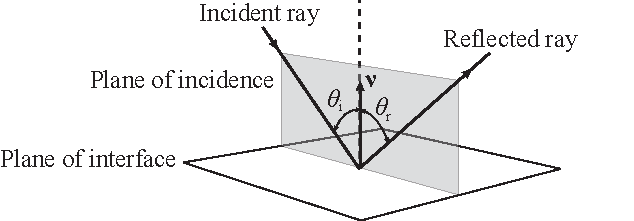
\includegraphics[width=10cm]{plane_of_incidence1}
     \end{center}
     \caption{\textbf{Light ray that hits a mirror located on the reflecting plane.} The incident and the reflected ray are coplanar with the normal to the mirror. The plane of incidence is spanned by the reflected and the refracted rays. The plane of interface is perpendicular to the plane of incidence.}
\label{fig:planeofincidence}
 \end{figure}
The light polarization can be classified into three different kinds of polarization:
\begin{itemize}
\item \textit{Linear polarization}: The electric filed is confined to a single plane perpendicular to the direction of propagation;
\item \textit{Circular polarization}: The electric field describes a circle around the direction of propagation;
\item \textit{Elliptic polarization}: The electric field describes an ellipse around the direction of propagation.
\end{itemize}
Any form of light can be defined by two orthogonal linear polarizations.
Hence, the following two cases of light polarization are considered: 
\begin{enumerate}
\item $\boldsymbol{\mathcal{E}}$ is perpendicular to the plane of incidence, and therefore $\boldsymbol{\mathcal{B}}$ is parallel to it (see Figure \ref{fig:electric_field}). In this case light is said to be \textit{s-polarized} (from the German word \textit{senkrecht}).
\item $\boldsymbol{\mathcal{E}}$ is parallel to the plane of incidence and, therefore $\boldsymbol{\mathcal{B}}$ is perpendicular to it (see Figure \ref{fig:electric_field_p}). In this case light is said to be \textit{p-polarized} (from the German word \textit{parallel}).
\end{enumerate}
\begin{figure}[t]
 \label{fig:electric_field}
     \begin{center}
     \includegraphics[width=8cm]{electric_field}
     \end{center}
     \caption{\textbf{Propagation of an electromagnetic wave for s-polarized light.} The components of $\boldsymbol{\mathcal{E}}$ are indicated with the green circles.
The components of $\boldsymbol{\mathcal{B}}$ are indicated with red arrows.}
\label{fig:electric_field}
 \end{figure}
\begin{figure}[t]
 \label{fig:electric_field_p}
     \begin{center}
     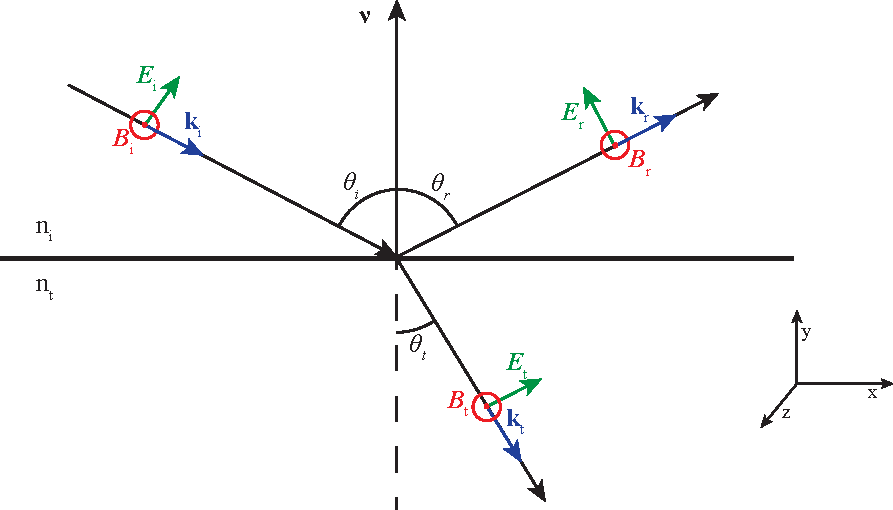
\includegraphics[width=8cm]{electric_field_p}
     \end{center}
 \caption{\textbf{Propagation of an electromagnetic wave for p-polarized light.} The components of $\boldsymbol{\mathcal{B}}$ are indicated with the red circle.
%, they are in the $(\variabile{x},\variabile{z})$ plane and they are oriented in the positive direction of $\variabile{z}$. 
The components of $\boldsymbol{\mathcal{E}}$ are indicated with green arrows.}
%and they are located in the $(\variabile{x}, \variabile{z})$ plane.}
\label{fig:electric_field_p}
 \end{figure}
The amplitude Fresnel coefficient $r$ is defined by the ratio between the amplitudes of the reflected and the incident electric field. Similarly, $t$ is the ratio between the amplitudes of the transmitted and the incident electric field. They are defined by:
\begin{equation}
\begin{split}
r & =\frac{|\boldsymbol{\mathcal{E}}_{0 \textrm{r}}|}{|\boldsymbol{\mathcal{E}}_{0\textrm{i}}|}, \\
t & =\frac{|\boldsymbol{\mathcal{E}}_{0 \textrm{t}}|}{|\boldsymbol{\mathcal{E}}_{0\textrm{i}}|}.
\end{split}
\end{equation}
The Fresnel equations provide the perpendicular $r_\textrm{s}$ and $t_\textrm{s}$ and parallel $r_\textrm{p}$ and $t_\textrm{p}$ versions of $r$ and $t$, respectively.
Energy conservation gives the boundary conditions of the electromagnetic field at the plane of the interface (perpendicular to the incident plane), from which the Fresnel coefficients are derived. They are defined in both case $1$ and case $2$. Since the mathematical formulation is similar for the two cases, in the following we explain in detail the computation of the Fresnel coefficients only for s-polarized light (case $1$).\\ 
\indent For s-polarized light, the component tangential to the interface of $\boldsymbol{\mathcal{E}}$ and $\boldsymbol{\mathcal{B}}/\mu$ are continuous across the boundary between the two different media, where $\mu$ is the permeability of the material in which the electromagnetic field is located. From now on, all quantities defined in the medium of the incident, reflective and transmitted light are indicated with the subscripts \textrm{i}, \textrm{r} and \textrm{t}, respectively. The continuity of the tangential component of $\boldsymbol{\mathcal{E}}$ leads to:
\begin{equation}\label{Econservation}
|\boldsymbol{\mathcal{E}}_{0\textrm{i}}|+|\boldsymbol{\mathcal{E}}_{0\textrm{r}}|= |\boldsymbol{\mathcal{E}}_{0\textrm{t}}|,
\end{equation} 
%where we have indicated with $\mathcal{E}_{0\textrm{i}}$, $\mathcal{E}_{0\textrm{r}}$ and $\mathcal{E}_{0\textrm{t}}$
%the magnitudes of $\boldsymbol{\mathcal{E}}_{0\textrm{i}}$, $\boldsymbol{\mathcal{E}}_{0\textrm{r}}$ and $\boldsymbol{\mathcal{E}}_{0\textrm{t}}$, respectively.
while the continuity of the tangential component of $\boldsymbol{\mathcal{B}}/\mu$ gives:
\begin{equation}\label{Bconservation}
-\frac{|\boldsymbol{\mathcal{B}}_{0\textrm{i}}|}{\mu_\textrm{i}}\cos\myangle_{\textrm{i}}+\frac{|\boldsymbol{\mathcal{B}}_{0\textrm{r}}|}{\mu_\textrm{r}}\cos\myangle_{\textrm{r}} = 
-\frac{|\boldsymbol{\mathcal{B}}_{0\textrm{t}}|}{\mu_\textrm{t}}\cos\myangle_{\textrm{t}},
\end{equation}
where the sign convention is chosen as illustrated in Figure \ref{fig:electric_field}.
%where we have indicated with $\mathcal{B}_{\textrm{i}}$, $\mathcal{B}_{\textrm{r}}$ and $\mathcal{B}_{\textrm{t}}$
%the absolute values of $\boldsymbol{\mathcal{B}}_{\textrm{i}}$,$\boldsymbol{\mathcal{B}}_{\textrm{r}}$ and $\boldsymbol{\mathcal{B}}_{\textrm{t}}$, respectively.
Since $|\boldsymbol{\mathcal{B}}| = |\boldsymbol{\mathcal{E}}|/v$, (\ref{Bconservation}) can be written as 
\begin{equation}
\frac{1}{\mu_{\textrm{i}}v_{\textrm{i}}}(|\boldsymbol{\mathcal{E}}_{0\textrm{i}}|-|\boldsymbol{\mathcal{E}}_{0\textrm{r}}|)\cos\myangle_{\textrm{i}} = \frac{1}{\mu_{\textrm{t}}v_{\textrm{t}}}|\boldsymbol{\mathcal{E}}_{0\textrm{t}}|\cos\myangle_{\textrm{t}},
\end{equation}
where we employed the fact that $v_{\textrm{i}}= v_{\textrm{r}}$, and $\myangle_{\textrm{i}}= \myangle_{\textrm{r}}$. 
Since $n = c/v$, the previous equation becomes:
\begin{equation}
\frac{n_{\textrm{i}}}{\mu_{\textrm{i}}}(|\boldsymbol{\mathcal{E}}_{0\textrm{i}}|-|\boldsymbol{\mathcal{E}}_{0\textrm{r}}|)\cos\myangle_{\textrm{i}} = \frac{n_{\textrm{t}}}{\mu_{\textrm{i}}}|\boldsymbol{\mathcal{E}}_{0\textrm{t}}|\cos\myangle_{\textrm{t}}.
\end{equation}
Most often used optical materials are non-magnetic, hence we assume $\mu_{\textrm{i}}=\mu_{\textrm{t}}=\mu_{0}$ \cite{lvovsky2013fresnel}. Employing (\ref{Econservation}) we arriving at the Fresnel coefficients for s-polarized light:
\begin{equation} \label{Fresnel_perpendicular}
\begin{split}
r_{\textrm{s}} & =\frac{|\boldsymbol{\mathcal{E}}_{0 \textrm{r}}|_{\textrm{s}}}{|\boldsymbol{\mathcal{E}}_{0\textrm{i}}|_\textrm{s}} = 
\frac{n_\textrm{i}\cos\myangle_\textrm{i}-n_\textrm{t} \cos\myangle_\textrm{t}}{n_\textrm{i}
\cos\myangle_\textrm{i}+n_\textrm{t}\cos\myangle_\textrm{t}},\\
t_{\textrm{s}} & = \frac{|\boldsymbol{\mathcal{E}}_{0 \textrm{t}}|_\textrm{s}}{|\boldsymbol{\mathcal{E}}_{0\textrm{i}}|_\textrm{s}} 
=\frac{2\n_\textrm{i}\cos\myangle_\textrm{i}}{n_\textrm{i}\cos\myangle_\textrm{i}+\n_\textrm{t}\cos\myangle_\textrm{t}},\\
\end{split}
\end{equation}
where the subscript $\textrm{s}$ is used to remind the reader that we are considering s-polarized light. 
Using Snell's law (Equation (\ref{eq:snell})) the first pair of the Fresnel equations restricted to the case $\myangle_\textrm{i}\leq\myangle_\textrm{c}$ becomes:
\begin{equation}
\fbox{\begin{minipage}{18em}
\begin{equation*} \label{simple_Fresnel}
\begin{split}
r_{\textrm{s}} & = -\frac{\sin(\myangle_\textrm{i}-\myangle_\textrm{t})}{\sin(\myangle_\textrm{i}+\myangle_\textrm{t})}\\
t_{\textrm{s}} & = \frac{2\sin \myangle_\textrm{t} \cos \myangle_\textrm{i}}{\sin(\myangle_\textrm{i}+\myangle_\textrm{t})}
\end{split}
\end{equation*}
\end{minipage}}
\end{equation}

A similar argument for p-polarized light leads to the calculation of the parallel versions $r_\textrm{p}$ and $t_\textrm{p}$ of $r$ and $t$. 
The boundary conditions for the electric and magnetic field read:
\begin{subequations}
\begin{align}
|\boldsymbol{\mathcal{E}}_{0 \textrm{i}}|\cos\myangle_{\textrm{i}} - |\boldsymbol{\mathcal{E}}_{0 \textrm{r}}|\cos\myangle_{\textrm{r}} &= 
|\boldsymbol{\mathcal{E}}_{0 \textrm{t}}|\cos\myangle_{\textrm{t}}\\
|\boldsymbol{\mathcal{B}}_{0 \textrm{i}}| + 
|\boldsymbol{\mathcal{B}}_{0 \textrm{r}}| &= 
|\boldsymbol{\mathcal{B}}_{0 \textrm{t}}|,
\end{align}
\end{subequations}
leading to the second pair of Fresnel's equations:
\begin{equation}\label{Fresnel_parallel}
\begin{split}
r_{\textrm{p}} & = \frac{|\boldsymbol{\mathcal{E}}_{0 \textrm{r}}|_{\textrm{p}}}{|\boldsymbol{\mathcal{E}}_{0\textrm{i}}|_\textrm{p}} = \frac{\n_\textrm{t}\cos\myangle_\textrm{i}-n_\textrm{i} \cos\myangle_\textrm{t}}{n_\textrm{i} \cos\myangle_\textrm{t}+n_\textrm{t}\cos\myangle_\textrm{i}},\\
t_{\textrm{p}} & =\frac{|\boldsymbol{\mathcal{E}}_{0 \textrm{t}}|_{\textrm{p}}}{|\boldsymbol{\mathcal{E}}_{0\textrm{i}}|_\textrm{p}} =  \frac{2\n_\textrm{i}\cos\myangle_\textrm{i}}{n_\textrm{i}\cos\myangle_\textrm{t}+n_\textrm{t}\cos\myangle_\textrm{i}}.
\end{split}
\end{equation}
%where $\myangle_\textrm{i}\leq\myangle_\textrm{c}$. 
Similarly to the $s$-polarized case, using Snell's law, the previous equations when $\myangle_\textrm{i}\leq\myangle_\textrm{c}$ reduce to:
\begin{equation}
\fbox{\begin{minipage}{18em}
\begin{equation*} \label{simple_Fresnel_p}
\begin{split}
r_{\textrm{p}} & =  \frac{\tan(\myangle_\textrm{i}-\myangle_\textrm{t})}{\tan(\myangle_\textrm{i}+\myangle_\textrm{t})}\\
t_{\textrm{p}} & = \frac{2\sin \myangle_\textrm{t} \cos \myangle_\textrm{i}}{\sin(\myangle_\textrm{i}+\myangle_\textrm{t})\cos(\myangle_\textrm{i}- \myangle_\textrm{t})}
\end{split}
\end{equation*}
\end{minipage}}
\end{equation}
Furthermore, it can be checked that
 \begin{equation}
t_\textrm{s}-r_\textrm{s} = 1
\end{equation}
holds for every $\myangle_{\textrm{i}}$, while 
\begin{equation}
t_\textrm{p}+r_\textrm{p} =  1
\end{equation}
is valid only at normal incidence ($\myangle_{\textrm{i}} = 0$).
\\ \indent The amplitude coefficients are shown in Figure \ref{fig:coefficients} for the case in which light travels from a less dense to a more dense medium, i.e., $\n_\textrm{i}<n_\textrm{t}$ where $\n_{\textrm{i}}= 1$ and $\n_{\textrm{t}}=1.5$, thus $\myangle_\textrm{i}>\myangle_\textrm{t}$. 
In Figure \ref{fig:coefficients2} the amplitude coefficients are shown for the case in which $\n_\textrm{i}>n_\textrm{t}$ with $\n_{\textrm{i}}= 1.5$ and $\n_{\textrm{t}}=1$ ($\myangle_\textrm{i}<\myangle_\textrm{t}$). Note, from Figure \ref{fig:coefficients} that $r_\textrm{p}$ approaches $0$ when $\myangle_\textrm{i}$ approaches $\myangle_\textrm{p}$ and it gradually decreases, reaching $-1$ for an incident angle $\myangle_\textrm{i}=90^\circ$. The angle $\myangle_\textrm{p}$ is called \textit{Brewster's angle} or polarization angle as only the component perpendicular to the incident plane is reflected at that angle and therefore light is perfectly polarized. Similarly, Figure \ref{fig:coefficients2} shows that $r_\textrm{p}=0$ for $\myangle_\textrm{i}= \myangle_{\textrm{p}\prime}$. It can be show that $\myangle_\textrm{p}+ \myangle_{\textrm{p}\prime}= 90^\circ$. Both $r_\textrm{p}$ and $r_\textrm{s}$ reach $1$ when $\myangle_\textrm{i}~=~\myangle_\textrm{c}$. $\myangle_\textrm{c}$ is called the critical angle. Light that hits the incident plane with an incident angle equal to or greater than $\myangle_{\textrm{c}}$ is totally reflected back and no transmitted light is observed. This phenomenon is called total internal reflection. 
\begin{figure}[t]
  \begin{minipage}[h]{0.48\textwidth}
    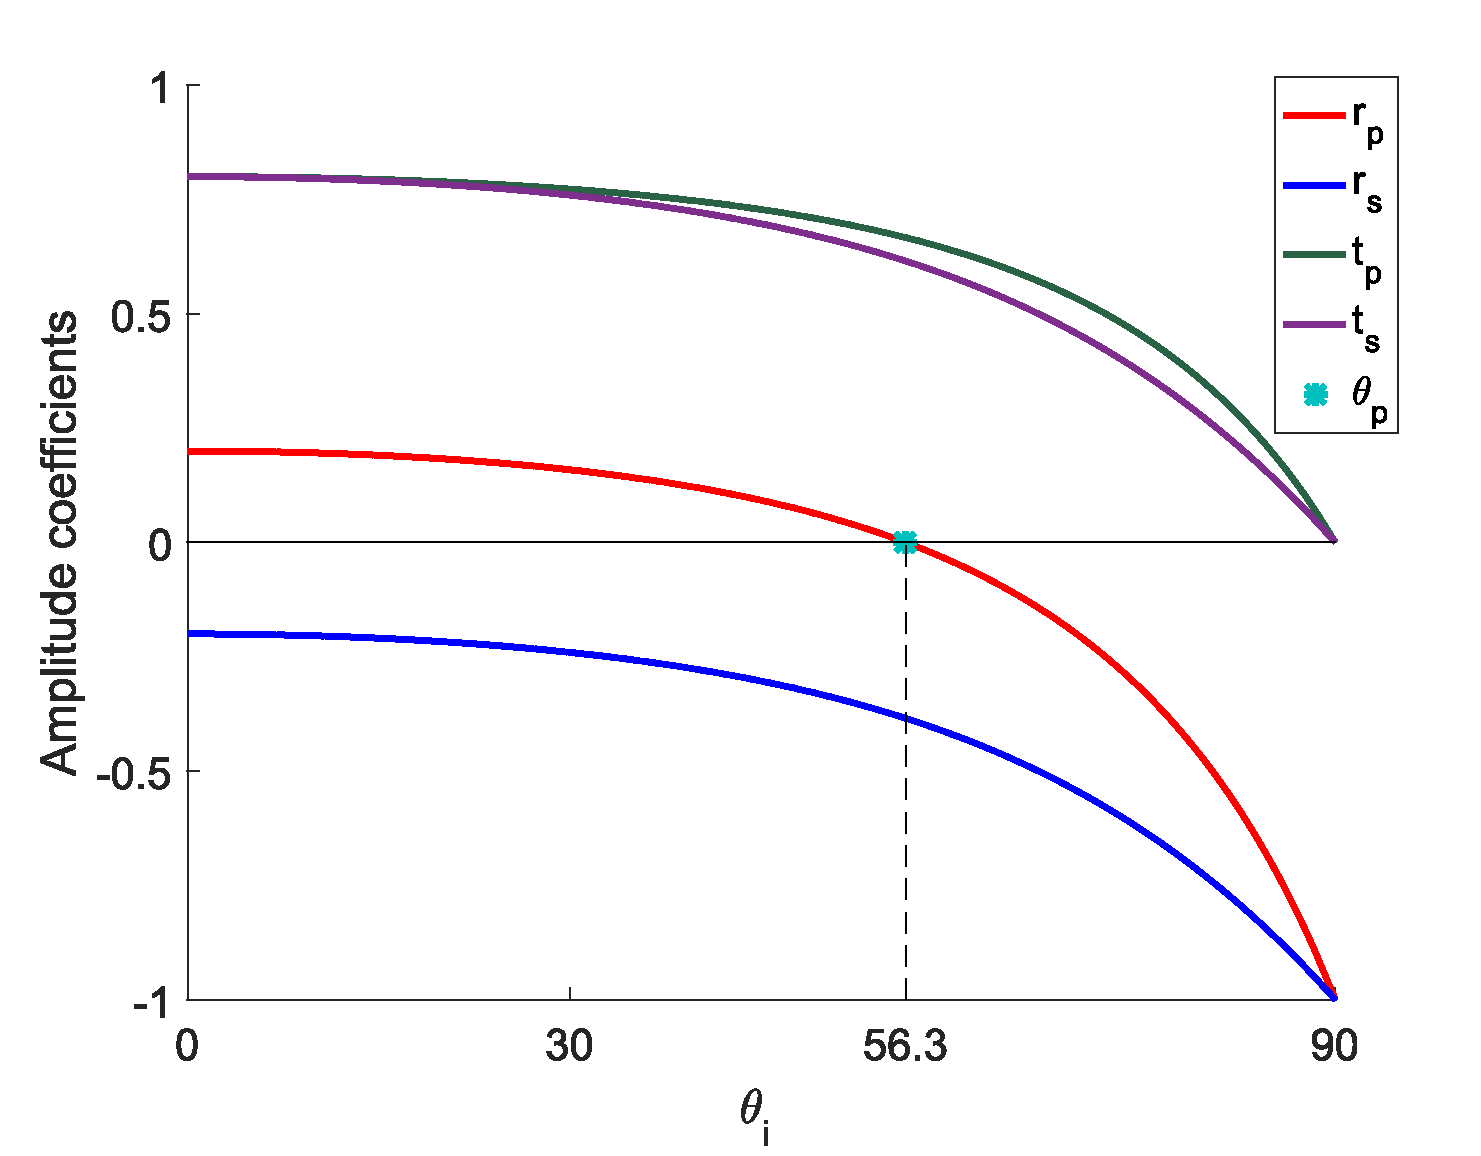
\includegraphics[width=\textwidth]{amplitude_coefficients}
    \caption{\textbf{Amplitude coefficients of reflection and transmission.} $n_\textrm{i}<n_\textrm{t}$
($n_\textrm{i} = 1$ and $\n_\textrm{t}=1.5$). $\myangle_\textrm{p} ~=~ 56.3^\circ$ is the polarization angle.}
    \label{fig:coefficients}
  \end{minipage}\hfill
  \begin{minipage}[h]{0.48\textwidth}
    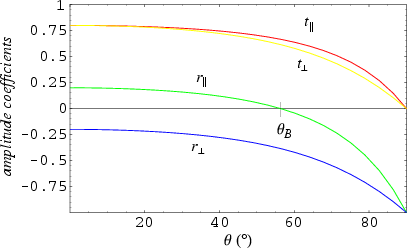
\includegraphics[width=\textwidth]{amplitude_coefficients3}
    \caption{\textbf{Amplitude coefficients.} $n_\textrm{i}>n_\textrm{t}$
($n_\textrm{i} = 1.5$ and $n_\textrm{t}=1$). $\myangle_{p\prime}~=~ 33.7^\circ$ is the polarization angle and $\myangle_\textrm{c}= 41.8^\circ$ is the critical angle.}
   \label{fig:coefficients2}
 \end{minipage}
\end{figure}\\
%\indent The  we introduce the Poynting vector \vect{P} that defines the energy flux of an electromagnetic field. 
%It is measured in $[\textrm{W}/\textrm{m}^2]$, and it is given by:
%\begin{equation}
%\vect{P} = \frac{1}{\mu}\Big(\boldsymbol{\mathcal{E}}\boldsymbol{\times} \boldsymbol{\mathcal{B}}\Big),
%\end{equation}
%where $\mu = \frac{1}{\varepsilon v^2}$ is the permeability and $\varepsilon$ the permittivity of the medium.
% In the following, the parameters for vacuum are indicated with the subscript $0$. Optical rays are perpendicular to the wave front of an electromagnetic wave and parallel to the Poynting vector \cite{jones2015optical}.
\indent To calculate the amount of energy reflected and transmitted, it is necessary to define the reflection and transmission coefficients in terms of the irradiance (or radiant flux density) $P$ rather than in terms of amplitudes of the electric field. For a wave of amplitude $|\boldsymbol{\mathcal{E}}_0|$ propagating in a non-magnetic medium with a refractive index $n$, the energy flux $P$ is given by:
%Therefore, defining the average of the vector \vect{P} over the time as:
%\begin{equation}
%\langle \vect{P} \rangle_T = \frac{1}{T}\int_0^T \vect{P}\textrm{d}T
%\end{equation}
%we can write the irradiance $E$ as:
\begin{equation}
P = \frac{c\, n \, \varepsilon_0}{2}|\boldsymbol{\mathcal{E}}_0|^2,
\end{equation}
\cite{hecht1998hecht}. For a beam of light that hits a surface such that an area $A$ is illuminated,
$P$ is the average energy that crosses in unit time a unit area $A$ perpendicular to the direction of the energy flow.
We indicate with $P_{\textrm{i}}$, $P_{\textrm{r}}$ and $P_{\textrm{t}}$ the incident, reflected and transmitted flux densities, respectively.
The energy per unit time for the incident, reflected and transmitted beams are 
$P_\textrm{
i} A\cos\myangle_\textrm{i}$, $P_\textrm{r} A\cos\myangle_\textrm{r}$, and 
$P_\textrm{t} A\cos\myangle_\textrm{t}$, respectively. % as is shown in Figure \ref{}
The reflectance $\mathcal{R}$ is the ratio of the reflected power to the incident power:
\begin{equation}\label{reflectance}
\mathcal{R} = \frac{P_\textrm{r}\cos\myangle_\textrm{r}}{P_\textrm{i}\cos\myangle_\textrm{i}} = \frac{|\boldsymbol{\mathcal{E}}_{0 \textrm{r}}|^2}{|\boldsymbol{\mathcal{E}}_{0 \textrm{i}}|^2} = r^2,
\end{equation}
where the second equality holds because $\n_{\textrm{i}}= \n_{\textrm{r}}$, $\varepsilon_{\textrm{i}} = \varepsilon_{\textrm{r}}$ and $\myangle_{\textrm{i}} = \myangle_{\textrm{r}}$.
Similarly, the transmittance $\mathcal{T}$ is the ratio between the transmitted to the incident power:
\begin{equation}\label{transmittance}
\mathcal{T} = \frac{P_\textrm{t} \cos\myangle_\textrm{t}}{P_\textrm{i}\cos\myangle_\textrm{i}} = \frac{n_\textrm{t} \cos\myangle_\textrm{t}}{n_\textrm{i} \cos\myangle_\textrm{i}}\frac{|\boldsymbol{\mathcal{E}}_{0 \textrm{t}}|^2}{\boldsymbol{|\mathcal{E}}_{0 \textrm{i}}|^2} = \frac{n_\textrm{t} \cos\myangle_\textrm{t}}{n_\textrm{i} \cos\myangle_\textrm{i}} t^2\,.
\end{equation}
Employing total energy conservation, that is:
\begin{equation}
P_\textrm{i} A\cos\myangle_\textrm{i} = P_\textrm{r} A\cos\myangle_\textrm{r}+P_\textrm{t} A\cos\myangle_\textrm{t},
\end{equation}
we can easily prove that:
\begin{equation}
\fbox{\begin{minipage}{10em}
\begin{equation*}
\mathcal{R}+\mathcal{T}=1\,.
\end{equation*}
\end{minipage}}
\end{equation}
 The perpendicular and parallel versions of $\mathcal{R}$ and $\mathcal{T}$ are given by:
\begin{equation}
\fbox{\begin{minipage}{15em}
\begin{equation*}\label{Fresnel_pands}
\begin{split}
\mathcal{R}_\textrm{s} &=  r_\textrm{s}^2\\
\mathcal{T}_\textrm{s} &= \frac{n_\textrm{t} \cos\myangle_\textrm{t}}{n_\textrm{i} \cos\myangle_\textrm{i}}t_\textrm{s}^2\\
\mathcal{R}_\textrm{p}& =  {r_\textrm{p}^2}\\
\mathcal{T}_\textrm{p} &=  \frac{n_\textrm{t} \cos\myangle_\textrm{t}}{n_\textrm{i} \cos\myangle_\textrm{i}}t_\textrm{p}^2\\
\end{split}
\end{equation*}
\end{minipage}}
\end{equation}
It can be shown that 
%\begin{equation}
%\fbox{\begin{minipage}{15em}
\begin{equation}
\begin{split}
\mathcal{R}_\textrm{s}+\mathcal{T}_\textrm{s} &= 1,\\
\mathcal{R}_\textrm{p}+\mathcal{T}_\textrm{p} &=1\,.
\end{split}
\end{equation}
%\end{minipage}}
%\end{equation}
For normal incidence, i.e., $\myangle_\textrm{i} = 0$, the incident plane is not defined and there is no distinction between the perpendicular and the parallel versions of $\mathcal{R}$ and $\mathcal{T}$. As a consequence, (\ref{Fresnel_pands}) combined with (\ref{Fresnel_perpendicular}) and (\ref{Fresnel_parallel}) leads to:
\begin{equation}\label{eq:fresnel_pands2}
\begin{split}
\mathcal{R} &= \mathcal{R}_\textrm{p} = \mathcal{R}_\textrm{s} = \Bigg(\frac{n_\textrm{i}-n_\textrm{t}}{n_\textrm{t}+n_\textrm{i}}\Bigg)^2, \\
\mathcal{T} &= \mathcal{T}_\textrm{p} = \mathcal{T}_\textrm{s} = \frac{4n_\textrm{i} n_\textrm{t}}{(n_\textrm{t}+n_\textrm{i})^2}\,.
\end{split}
\end{equation}
%In two dimensions light hits lines instead of surfaces. Therefore only the plane of incidence is defined and it has no sense to consider separately the parallel and the perpendicular polarization. 
%If $\mathcal{R}_\textrm{p} = \mathcal{R}_\textrm{s}$ and $\mathcal{T}_\textrm{p} = \mathcal{T}_\textrm{s}$, then the amount of energy in both polarization states is the same \cite{hecht1998hecht}.\\ \indent

Many common light sources such as the sun, halogen lighting, LED spotlights, and incandescent bulbs produce unpolarized light. 
In this case, light can be represented by the sum of two orthogonal states. For unpolarized light, the convention is to take as reflectance and transmittance the averages:
\begin{equation}
\fbox{\begin{minipage}{15em}
\begin{equation*}\begin{split}
\mathcal{R} &= \frac{\mathcal{R}_\textrm{p}+ \mathcal{R}_\textrm{s}}{2}\\
\mathcal{T} &= \frac{\mathcal{T}_\textrm{p}+ \mathcal{T}_\textrm{s}}{2}
\end{split}
\label{eq:RandTin2D}
\end{equation*}
\end{minipage}}
\end{equation}
where $\mathcal{R}_\textrm{p}$, $\mathcal{R}_\textrm{s}$, $\mathcal{T}_\textrm{p}$ and $\mathcal{T}_\textrm{s}$ are obtained from (\ref{Fresnel_pands}). The reflectance $\mathcal{R}$ and the transmittance $\mathcal{T}$ give the fraction of the power of energy reflected and transmitted at every interaction of a light ray with a Fresnel surface.

With this overview we conclude this chapter. The notions given in Section \ref{sec:photometry} will be used in the entire thesis as our goal is to study the distribution of light at the target of some optical systems. In particular, we will focus on the computation of the output intensity distribution. The reflection and refraction laws explained in Section \ref{sec:reflection} are needed to determine how the optical system changes the ray's direction every time that it hits a surface (or a line in the two-dimensional case). In Chapters \ref{chap:raytracing}-\ref{chap:raymapping2} we restrict ourselves to pure reflection and refraction; the Fresnel reflection and refraction are ignored. Systems with Fresnel reflection is postponed until Chapter \ref{chap:fresnel}. The amount of reflected and transmitted light is calculated using (\ref{eq:RandTin2D}) and (\ref{Fresnel_pands}) where $r_\textrm{s}$ and $t_\textrm{s}$ are obtained from (\ref{Fresnel_perpendicular}) and $r_\textrm{p}$ and $t_\textrm{p}$ from (\ref{Fresnel_parallel}). In our simulations we consider the general case of unpolarized light. 
